\begin{figure}[htbp]
    \centering
    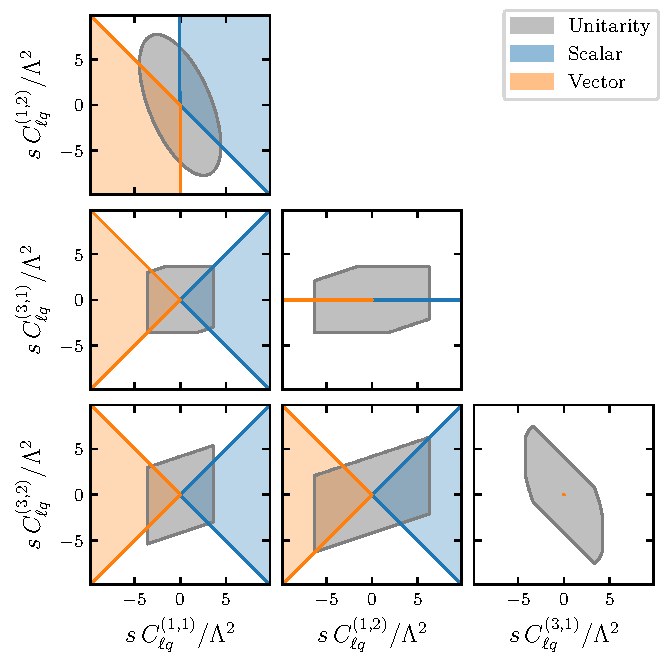
\includegraphics[scale = 0.75]{images/flavor/Olq_mfv.pdf}
    \caption{Partial-wave unitarity bounds and sum-rule constraints (under scalar and vector dominance) for the operators $O_{\ell q}^{(1,3)}$ under MFV, where $[C_{\ell q}^{(i)}]_{prst} =
            C_{\ell q}^{(i,1)}\delta_{pr}\delta_{st}
            + C_{\ell q}^{(i,2)}\delta_{pr}(Y_u Y_u^\dagger)_{st}$, $i=1,3$. The regions shown are two-dimensional slices of the full allowed region, obtained by setting to zero all the independent coefficients other than the two displayed.}
    \label{fig:Olq_mfv}
\end{figure}

\begin{figure}[htbp]
    \centering
    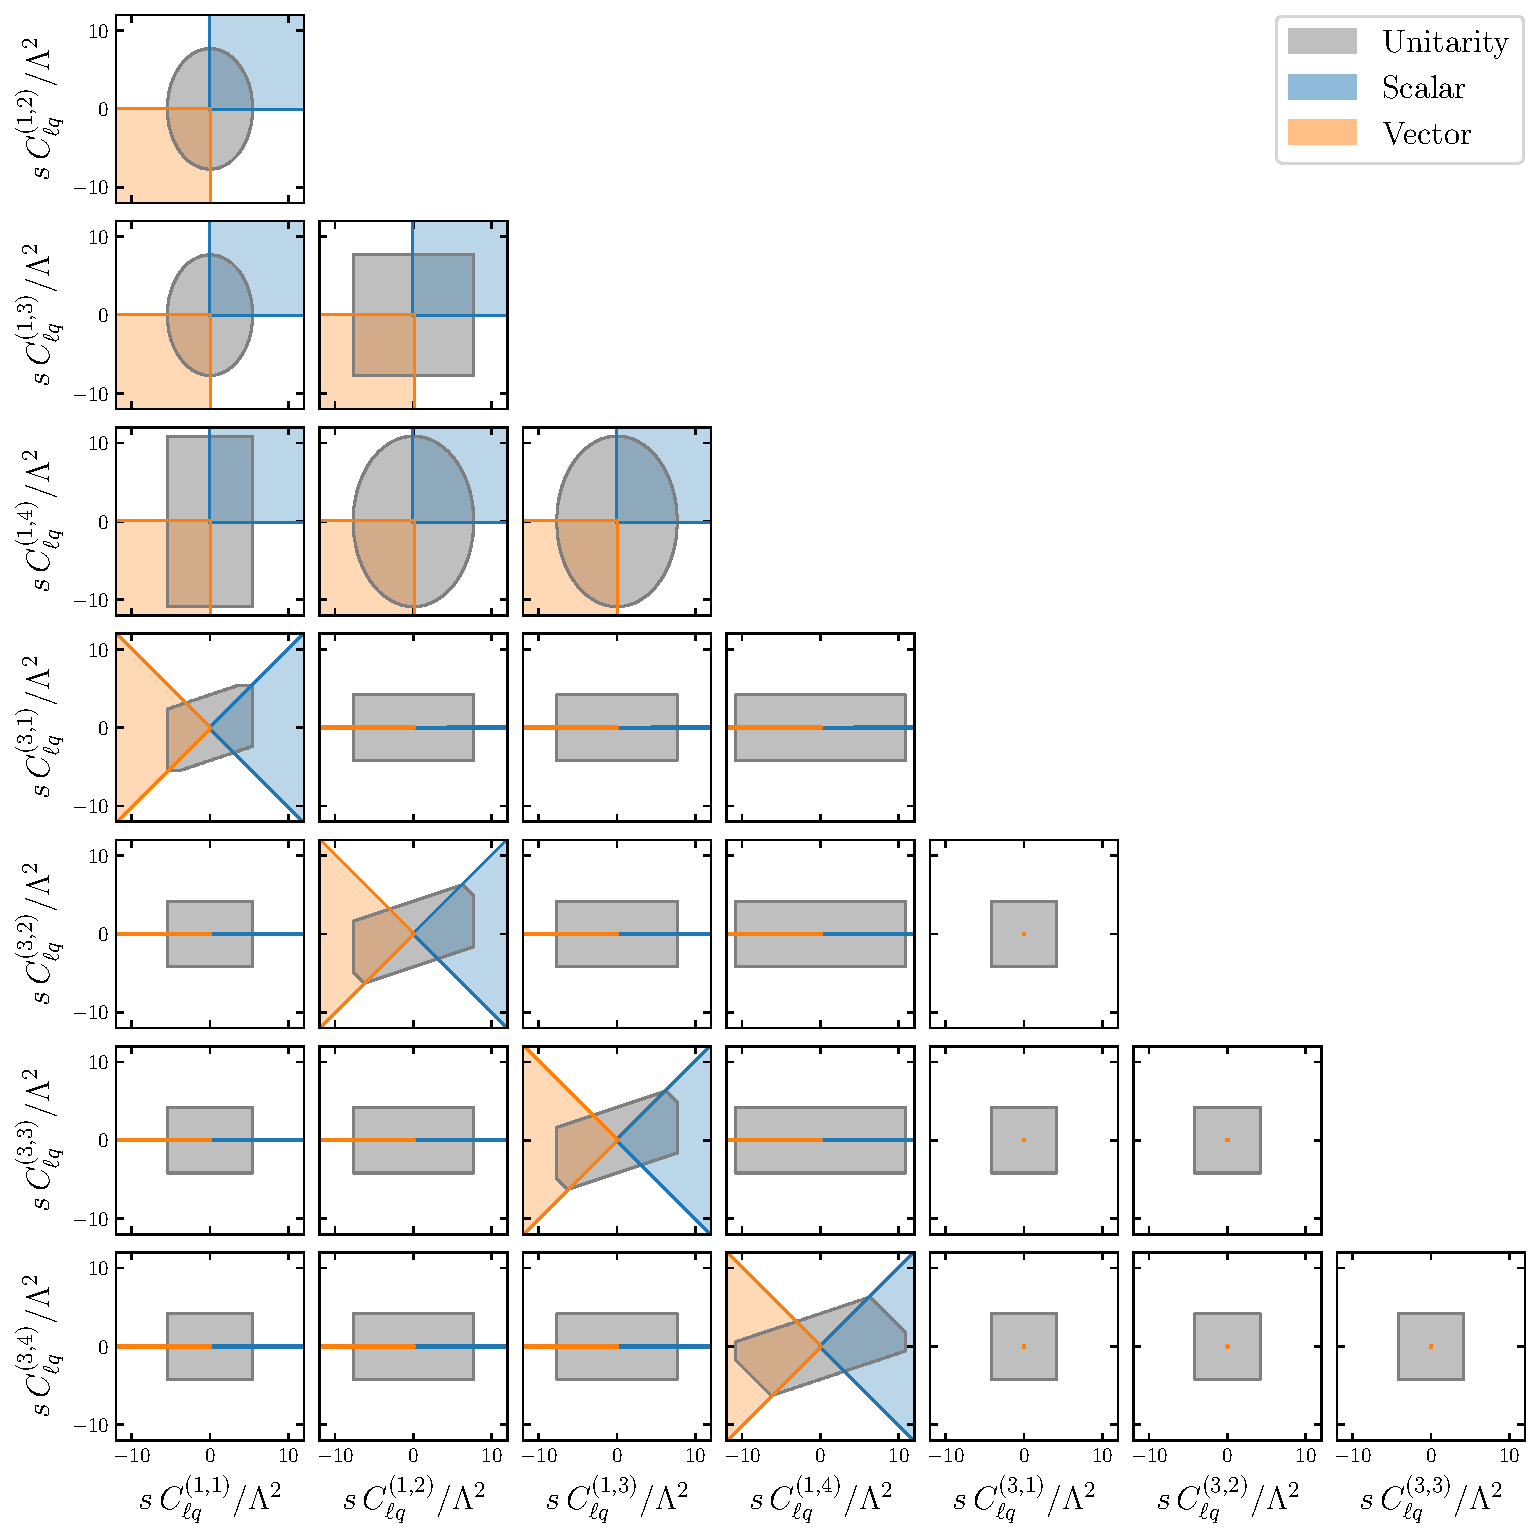
\includegraphics[width=1\linewidth]{images/flavor/Olq_u2.pdf}
    \caption{Partial-wave unitarity bounds and sum-rule constraints (under scalar and vector dominance) for the operators $O_{\ell q}^{(1,3)}$ under $U(2)^5$ flavor symmetry, where $[C_{\ell q}^{(i)}]_{prst} =
            C_{\ell q}^{(i,1)}\Pij{p}{r}{a}\Pij{s}{t}{b}
            + C_{\ell q}^{(i,2)}\delta_{p3}\delta_{3r}\Pij{s}{t}{a}
            + C_{\ell q}^{(i,3)}\Pij{p}{r}{a}\delta_{s3}\delta_{3t}
            + C_{\ell q}^{(i,4)}\delta_{p3}\delta_{3r}\delta_{s3}\delta_{3t}$, $i=1,3$. The regions shown are two-dimensional slices of the full allowed region, obtained by setting to zero all the independent coefficients other than the two displayed.}
    \label{fig:Olq_u2}
\end{figure}
